\documentclass[12pt]{article}

\usepackage[hmargin=.65in, vmargin=.75in]{geometry}
\usepackage[citecolor=blue, colorlinks=True, linkcolor=blue, urlcolor=blue]{hyperref}
\usepackage{natbib}
\usepackage{graphicx}
\usepackage{multirow}
\usepackage{tabularx}
\usepackage[table, svgnames]{xcolor}
\usepackage{authblk}
\usepackage{booktabs}
\usepackage[toc,page]{appendix}
\usepackage[T1]{fontenc}
\usepackage{enumitem}
\usepackage{caption}

\title{A Standard for Exchangeable Magnetotelluric Metadata}
\date{\textbf{Version 0.0.1d -- June 2020}\footnote{\noindent\textbf{\textit{Corresponding Authors:}}
		
		Jared Peacock (\url{jpeacock@usgs.gov})
		
		Andy Frassetto (\url{andy.frassetto@iris.edu})}}
\author[1]{Working Group for Data Handling and Software - PASSCAL Magnetotelluric Program}
\affil[1]{Portable Array Seismic Studies of the Continental Lithosphere, Incorporated Research Institutions for Seismology}

\newcommand{\attr}[1]{\textbf{#1}}
\renewcommand{\arraystretch}{1.0}

\newcommand{\entry}[7]{
	\textbf{#1} 
	\begin{itemize}[topsep=5pt,itemsep=-.1pt,parsep=-2pt,partopsep=0pt,labelwidth=2em,align=left,itemindent=1em]
		\begin{small}
			\item[Required:] #2
			\item[Units:] #3
			\item[Type:] #4
			\item[Style:] #5
		\end{small}
	\end{itemize} & #6 & #7 \\ \midrule}

\begin{document}
	
\maketitle

\tableofcontents
\vspace{1cm}

\rowcolors{1}{white}{AliceBlue}

\newpage

\section{Introduction}

Researchers using magnetotelluric (MT) methods lack a standardized format for storing time series data and metadata. Commercially available MT instruments produce data in formats that range from proprietary binary to ASCII, and recent datasets from the U.S. MT community have utilized institutional formats or heavily adapted formats like miniSEED. In many cases, the available metadata for these time series are incomplete and only loosely standardized, and overall these datasets are not "user friendly". This lack of resources impedes the exchange and broader use of these data beyond a small community of specialists.

The \href{https://www.iris.edu/hq/programs/passcal/magnetotelluricnstrumentation}{IRIS PASSCAL MT facility} maintains a pool of MT instruments that are freely available to U.S. Principal Investigators (PIs). Datasets collected with these instruments are subject to data sharing requirements, and an IRIS \href{https://www.iris.edu/hq/aboutris/governance/mtoft}{working group} advises the development of sustainable data formats and workflows for this facility. Following in the spirit of the standard created for \href{https://library.seg.org/doi/10.1190/geo2018-0679.1}{MT transfer function} datasets, this document outlines a new metadata standard for MT time series. This standard is a key pillar of MTH5, a new data format which we propose for the international community of MT practitioners. Further information regarding MTH5 will be available later in 2020.

The Python 3 module written for these standards are found at \url{https://github.com/kujaku11/MTarchive/tree/tables}.

\section{General Structure}

The metadata for a full MT dataset are structured to cover details from single channel time series to the full survey. For simplicity each of the different scales of an MT survey and measurements have been categorized starting from largest to smallest (Figure \ref{fig:example}). These categories are: \verb|Survey|, \verb|Station|, \verb|Run|, \verb|DataLogger|, \verb|Electric Channel|, \verb|Magnetic Channel|, and \verb|Auxiliary Channels|. Each of these are described in subsequent sections.  Required keywords are labeled as \verb|True| and suggested keywords are labeled as \verb|False| a user should try to use as much of the suggested metadata as possible for a full description of the data.  

\begin{figure}[htb!]
	\centering
	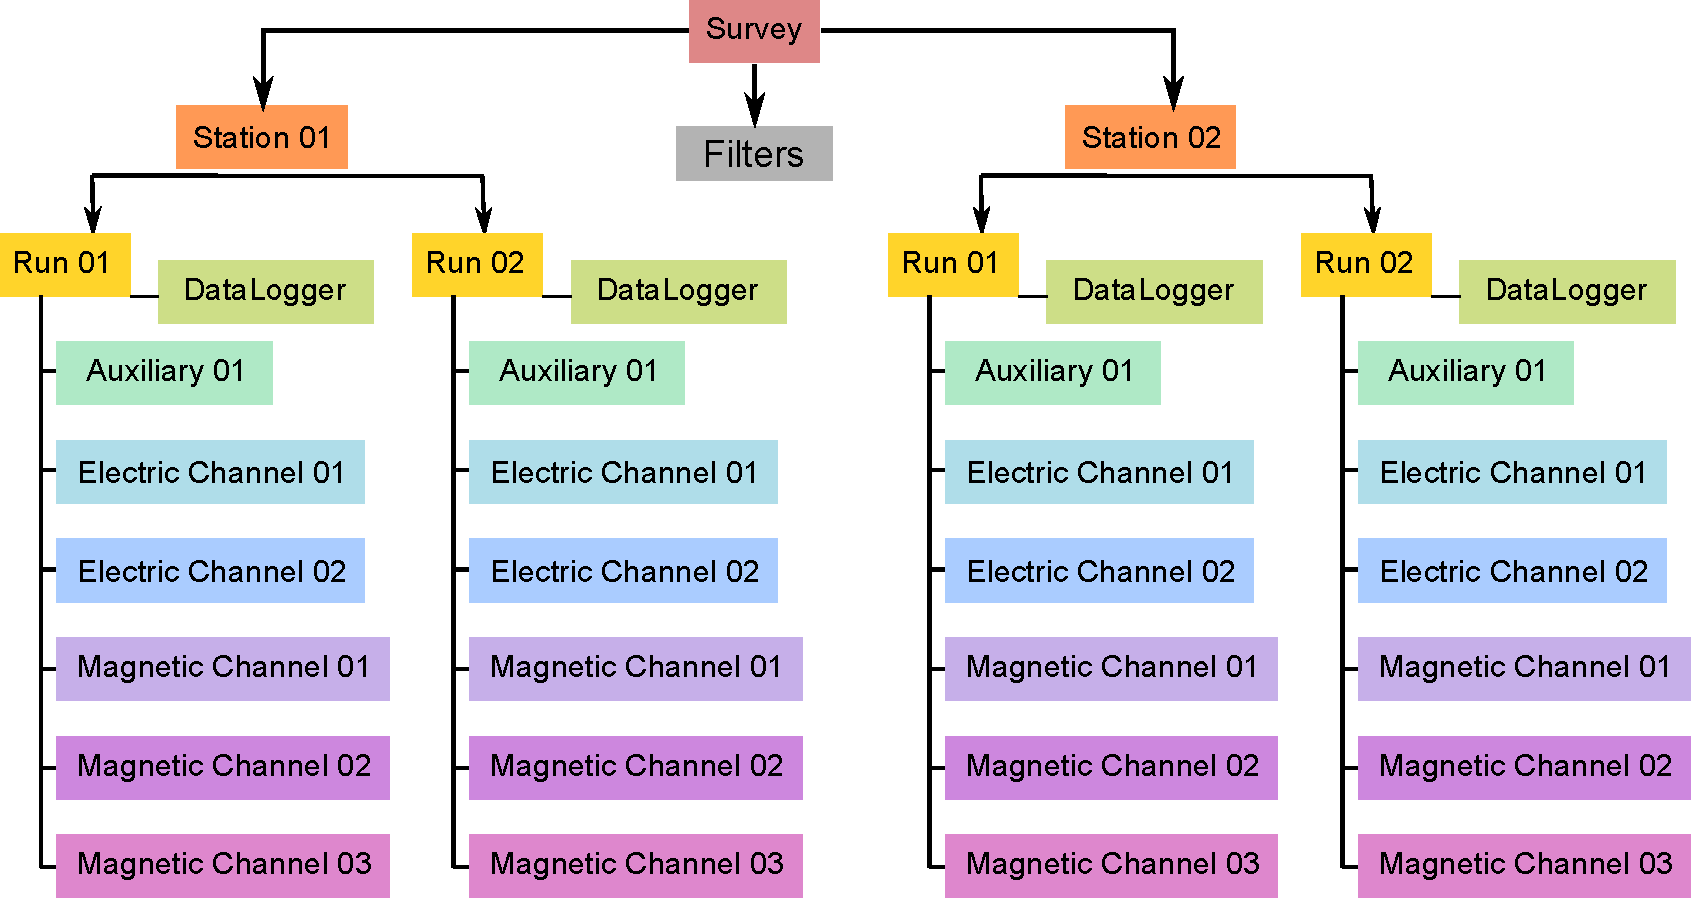
\includegraphics[height=.525\textwidth]{example_mt_file_structure.pdf}
	\caption{Schematic of a MT time series file structure with appropriate metadata. The top level is the \textit{Survey} that contains general information about who, what, when, where, how the data were collected.  Underneath \textit{Survey} are the \textit{Station} and \textit{Filter}.  \textit{Filter} contains information about different filters that need to be applied to the raw data to get appropriate units and calibrated measurements.  Underneath \textit{Station} are \textit{Run} which are blocks where data were collected at a single sampling rate with common start and end time. Finally \textit{Channel} which describes each channel of data collected, this can be an \textit{Auxiliary}, \textit{Electric}, or \textit{Magnetic}.  Metadata is attributed based on the type of data collected in the channel.}
	\label{fig:example}
\end{figure}

\subsection{Metadata Keyword Format}

The metadata key names should be self explanatory and they are structured as follows: \verb|{category}.{name}|, where:
\begin{itemize}
	\item \verb|category| refers to a metadata category that has common parameters, such as \verb|location| which will have a latitude, longitude, and elevation $\longrightarrow$ \verb|location.latitude|, \verb|location.longitude|, and \verb|location.elevation|.  These can be nested, for example \verb|positive.location.latitude|
	\item \verb|name| is a descriptive name, where words should be separated by an underscore. Note that only whole words should be used and abbreviations should be avoided. e.g. \verb|data_quality|.  
\end{itemize}  

As described in this document a '.' represents the separator between different categories.  The metadata can be stored in many different forms.  Common are XML or JSON formats.  See examples below for various ways to represent the metadata.      

\subsection{Formatting Standards}

Specific and required formatting standards for location, time and date, and angles are defined below and should be adhered to.

\subsubsection{Time and Date Format}

All time and dates are given as an ISO formatted date-time string in the UTC time zone.  The ISO date time format is \verb|YYYY-MM-DDThh:mm:ss.ms+00:00|, where UTC is represented by \verb|+00:00|. If the data requires a different time zone this can be accommodated but it is recommended that UTC be used whenever possible. Milliseconds can be accurate to 6 decimal places.  ISO dates are formatted \verb|YYYY-MM-DD|. 

\subsubsection{Location}

All latitude and longitude locations are given in decimal degrees in the well known datum specified at the \verb|Survey| level. \textbf{NOTE: The entire survey should use only one datum that is specified at the Survey level.}

\begin{itemize}
	\setlength\itemsep{0em}
	\item All latitude values must be $<|90|$ and all longitude values must be $<|180|$.
	\item Elevation and other distance values are given in meters.
	\item Datum should be one of the well known datums, WGS84 is preferred, but others are acceptable.
\end{itemize} 

\subsubsection{Angles}

All angles of orientation are given in decimal degrees.  Orientation of channels should be given in geographic coordinates where angles are assumed to be clockwise positive from Geographic North = 0.  If a station was collected not in geographic coordinates this needs to be specified in \verb|station.orientation.option| and the \verb|station.layout_rotation_angle| needs to be specified.   

\subsection{Units}
Acceptable units are only those from the International System of Units (SI).  Only long names in all lower case are acceptable.  Table \ref{tab:units} summarizes common acceptable units:


\begin{table}[!h]
	\centering
	\caption[Acceptable units]{Acceptable units}
	\begin{tabular}{ll}
		\toprule
		\textbf{Measurement Type} & \textbf{Unit Name} \\ \midrule
		Angles & degrees \\ \midrule
		
		Distance &  meters  \\ \midrule
		Latitude/Longitude & decimal degrees \\ \midrule
		Resistance & ohms   \\ \midrule
		Resistivity & ohm-meters \\ \midrule
		Temperature & celsius\\ \midrule
		Time & seconds\\ \midrule
		Voltage & volts \\ \bottomrule
		
		
	\end{tabular}
	\label{tab:units}
\end{table}

\subsection{String Formats}

Each metadata level has a column that describes the style of the input.  These are described in Table \ref{tab:values}.  Note that any list should be comma separated.

\begin{table}[htb!]
	\centering
	\caption[Acceptable String Formats]{Acceptable String Formats}
	\begin{tabular}{p{.8in}p{3.1in}c}
		\toprule
		\textbf{Style} & \textbf{Description}  & \textbf{Example} \\ \midrule
		free form & an unregulated string that can contain \{a-z, A-Z, 0-9\} and special characters & This is free form! \\ \midrule
		
		alpha numeric & a string that contains no spaces and only characters \{a-z, A-Z, 0-9, -, /, \_\} & WGS84 or GEOMAG-USGS \\ \midrule
		controlled vocabulary & Only certain names or words are allowed, in this case examples of acceptable values are provided in the documentation as [ option01 $|$ option02 $|$ ...]. The ... indicates that other options are possible but have not been defined yet. &  station.orientation.option = geographic \\ \midrule
		list & list of entries using a comma separator & 'Ex, Ey, Hx, Hy, Hz, T' \\ \midrule
		number & a number in the form of the data type, number of decimal places has not been implemented yet & 10.0 for float or 10 for int \\ \midrule
		date & ISO formatted date YYYY-MM-DD in UTC & 2020-02-02 \\ \midrule
		date time & ISO formatted date time YYYY-MM-DDThh:mm:ss.ms+00:00 in UTC & 2020-02-02T12:20:45.123456+00:00 \\ \midrule
		email & a valid email address & \url{person@mt.org} \\ \midrule
		url & a full URL that a user could put into a web browser  &  \url{https://www.passcal.nmt.edu/} \\ \bottomrule
		
		
	\end{tabular}
	\label{tab:values}
\end{table}

%\begin{table}[h!]
%	\centering
%	\caption[Attributes for Survey]{Attributes for Survey category}
%	\begin{tabular}{p{.25\textwidth}p{.6\textwidth}p{.15\textwidth}}
%		\hline
%		\textbf{Metadata Key} & \textbf{Description} & \textbf{Example} \\ \toprule
%		attribute
%		\begin{itemize}[noitemsep,topsep=0pt,parsep=0pt,partopsep=0pt,labelwidth=2em,align=left,itemindent=1em]
%			\item[Units:] None
%			\item[Type:] float
%			\item[Required:] True
%			\item[Style:] free form
%		\end{itemize} & A survey describes an entire data set that covers a specific time span and region. This may include multiple PIs in multiple data collection episodes but should be confined to a specific experiment. & this is an exampe \\ \midrule
%		\entry{attribute}{none}{boolean}{True}{bool}{description}{false}
%	\end{tabular}
%\end{table}

\clearpage
\newpage
\section{Survey}

A survey describes an entire data set that covers a specific time span and region. This may include multiple PIs in multiple data collection episodes but should be confined to a specific experiment. The \verb|Survey| metadata category describes the general parameters of the survey.

\begin{table}[h!]
	\caption[Attributes for Survey]{Attributes for Survey Category}
	\begin{tabular}{p{.275\textwidth}p{.5\textwidth}p{.2\textwidth}}
	\textbf{Metadata Key} & \textbf{Description} & \textbf{Example} \\ \toprule
	\entry{acquired\_by.author}{True}{None}{string}{free form}{Name of the person or persons who acquired the data.  This can be different from the project lead if a contractor or different group collected the data.}{person name}
	\entry{acquired\_by.comments}{False}{None}{string}{email}{Email of the contact person who acquired the data. This is in case there are any questions about aspects of how the data were collected or any inconsistencies in the data.}{expert digger}
	\entry{archive\_id}{True}{None}{string}{alpha numeric}{Alphanumeric name provided by the archive.  For IRIS this will be a 5 character string.}{YKN20}
	\entry{archive\_network}{True}{None}{string}{alpha numeric}{Network code given by PASSCAL/IRIS/FDSN.  This will be a two character string that describes who and where the network operates.}{EM}
	\entry{citation\_dataset.doi}{True}{None}{string}{url}{The full url of the doi number provided by the archive that describes the raw data}{\url{http://doi.10.adfabe}}
	\entry{citation\_journal.doi}{True}{None}{string}{url}{The full url of the doi number for a journal article(s) that uses these data.  If multiple journal articles use these data provide as a comma separated string of urls. }{\url{http://doi.10.xbsfs}, or \url{http://doi.10.xbsfs}, \url{http://doi.10.xbsfs2}}
	\end{tabular}
	\label{tab:survey}
\end{table} 

\clearpage
\newpage

\begin{table}[h!]
	\caption*{Attributes for Survey Category Continued}
	\begin{tabular}{p{.305\textwidth}p{.47\textwidth}p{.2\textwidth}}
		\textbf{Metadata Key} & \textbf{Description} & \textbf{Example} \\ \toprule
		\entry{comments}{True}{None}{string}{free form}{Any comments about the survey that are important for any user to know.}{Solar activity low.}	
		\entry{country}{True}{None}{string}{free form}{Country(s) countries that the survey is located in. If multiple input as comma separated names}{"USA, Canada"}
		\entry{datum}{True}{None}{string}{controlled vocabulary}{The reference datum for all geographic coordinates throughout the survey. It is up to the user to be sure that all coordinates are projected into this datum.  Should be a well-known datum: \qquad [ WGS84 $|$ NAD83 $|$ OSGB36 $|$ GDA94 $|$ ETRS89 $|$ PZ-90.11 $|$ other ].}{WGS84}
		\entry{geographic\_name}{True}{None}{string}{free form}{Geographic names that encompass the survey.  These should be broad geographic names.  Further information can be found at \url{https://www.usgs.gov/core-science-systems/ngp/board-on-geographic-names}}{Yukon}
		\entry{name}{True}{None}{string}{free form}{Descriptive name of the survey, similar to the title of a journal article.}{MT Characterization of Yukon Terrane}
		\entry{northwest\_corner.latitude}{True}{decimal degrees}{float}{number}{Latitude of the northwest corner of the survey in the datum specified.}{23.134}
		\entry{northwest\_corner.longitude}{True}{decimal degrees}{float}{number}{Longitude of the northwest corner of the survey in the datum specified.}{14.23}
	
	\end{tabular}
	\label{tab:survey2}
\end{table} 

\clearpage
\newpage

\begin{table}[h!]
	\caption*{Attributes for Survey Category Continued}
	\begin{tabular}{p{.305\textwidth}p{.47\textwidth}p{.2\textwidth}}
		\textbf{Metadata Key} & \textbf{Description} & \textbf{Example} \\ \toprule
		\entry{project}{True}{None}{string}{free form}{Alphanumeric name for the project.  This is different than the archive\_id in that it describes the overall project.  For example if the project is to estimate geomagnetic hazards that project may be GEOMAG but the survey could be YKN20, which will be the archive\_id.}{GEOMAG}
		\entry{project\_lead.author}{True}{None}{string}{free form}{author name}{Name the project lead.  This should be the person in charge who is responsible for the data.}		
		\entry{project\_lead.email}{True}{None}{string}{email}{Email of the project lead.  This is in case there are any questions about data.}{mt.guru@em.org}
		\entry{project\_lead.organization}{True}{None}{string}{free form}{Organization name of the project lead.}{MT Gurus}
		\entry{release\_status}{True}{None}{string}{controlled vocabulary}{How the data can be used. The options are based on Creative Commons (\url{https://creativecommons.org/licenses/}).  Options: \qquad [ CC0 $|$ CC BY $|$ CC BY-SA$|$ CC BY-ND $|$ CC BY-NC-SA $|$ CC BY-NC-ND]}{CC0}
		\entry{southeast\_corner.latitude}{True}{decimal degrees}{float}{number}{Latitude of the southeast corner of the survey in the datum specified.}{23.134}
		\entry{southeast\_corner.longitude}{True}{decimal degrees}{float}{number}{Longitude of the southeast corner of the survey in the datum specified.}{14.23}
		
	\end{tabular}
	\label{tab:survey3}
\end{table}

\clearpage
\newpage

\begin{table}[h!]
	\caption*{Attributes for Survey Category Continued}
	\begin{tabular}{p{.275\textwidth}p{.5\textwidth}p{.2\textwidth}}
		\textbf{Metadata Key} & \textbf{Description} & \textbf{Example} \\ \toprule
		\entry{summary}{True}{None}{string}{free form}{Summary paragraph of the survey including the purpose; difficulties; data quality; summary of outcomes if the data have been processed and modeled.}{Long project of characterizing mineral resources in Yukon}
		\entry{time\_period.end\_date}{True}{None}{string}{date}{End date of the survey in UTC.}{1995-02-01}
		\entry{time\_period.start\_date}{True}{None}{string}{date}{Start date of the survey in UTC.}{2020-06-21}
		
	\end{tabular}
	\label{tab:survey4}
\end{table}   

\clearpage
\newpage
\subsection{Example Survey XML Element}

\begin{verbatim}
<?xml version="1.0" ?>
<survey>
    <acquired_by>
        <author>MT Graduate Students</author>
        <comments>Multiple over 5 years</comments>
    </acquired_by>
    <archive_id>SAM1990</archive_id>
    <archive_network>EM</archive_network>
    <citation_dataset>
        <doi>https://doi.###</doi>
    </citation_dataset>
    <citation_journal>
        <doi>https://doi.###</doi>
    </citation_journal>
    <comments>None</comments>
    <country>USA, Canada</country>
    <datum>WGS84</datum>
    <geographic_name>Yukon</geographic_name>
    <name>Imaging Gold Deposits of the Yukon Province</name>
    <northwest_corner>
        <latitude type="float" units="decimal degrees">-130</latitude>
        <longitude type="float" units="decimal degrees">75.9</longitude>
    </northwest_corner>
    <project>AURORA</project>
    <project_lead>
        <email>m.tee@mt.org</email>
        <organization>EM Ltd.</organization>
        <author>M. Tee</author>
    </project_lead>
    <release_status>CC0</release_status>
    <southeast_corner>
        <latitude type="float" units="decimal degrees">-110.0</latitude>
        <longitude type="float" units="decimal degrees">65.12</longitude>
    </southeast_corner>
    <summary>This survey spanned multiple years with graduate students
             collecting the data.  Lots of curious bears and moose,
             some interesting signal from the aurora.  Modeled data
             image large scale crustal features like the 
             "fingers of god" that suggest large mineral deposits.
    </summary>
    <time_period>
        <end_date>1995-01-01</end_date>
        <start_date>2020-01-01</start_date>
    </time_period>
</survey>
\end{verbatim}

\clearpage
\newpage
\section{Station}

A station encompasses a single site where data are collected. If the location changes during a run, then a new station should be created and subsequently a new run under the new station. If the sensors, cables, data logger, battery are replaced during a run but the station remains stations, then this can be recorded in the \verb|Run| metadata but does not require a new station entry.

\begin{table}[h!]
	\caption[Attributes for Station Category]{Attributes for Station Category}
	\begin{tabular}{p{.305\textwidth}p{.47\textwidth}p{.2\textwidth}}
		\textbf{Metadata Key} & \textbf{Description} & \textbf{Example} \\ \toprule
		\entry{acquired\_by.author}{True}{None}{string}{free form}{Name of person or group that collected the station data and will be the point of contact if any questions arise about the data.}{person name}
		\entry{acquired\_by.comments}{False}{None}{string}{email}{Email of the contact person who collected the data for the station.}{expert digger}
		\entry{archive\_id}{True}{None}{string}{alpha numeric}{Station name that is archived {a-z;A-Z;0-9}.  For IRIS this is a 5 character string.}{MT201}
		\entry{channel\_layout}{False}{None}{string}{controlled vocabulary}{How the dipoles and magnetic channels of the station were laid out.  Options: [ L $|$ + $|$ other]}{+}
		\entry{channels\_recorded}{True}{None}{string}{controlled vocabulary}{List of components recorded by the station. Should be a summary of all channels recorded dropped channels will be recorded in Run.  \qquad Options: [ Ex $|$ Ey $|$ Hx $|$ Hy $|$ Hz $|$ T $|$ Battery $|$ other ]}{ Ex, Ey, Hx, Hy, Hz, T}
		\entry{comments}{False}{None}{string}{free form}{Any comments on the station that would be important for a user.}{Pipeline near by.}
	\end{tabular}
	\label{tab:station}
\end{table}


\clearpage
\newpage
\begin{table}[h!]
	\caption*{Attributes for Station Category Continued}
	\begin{tabular}{p{.305\textwidth}p{.47\textwidth}p{.2\textwidth}}
		\textbf{Metadata Key} & \textbf{Description} & \textbf{Example} \\ \toprule
		\entry{data\_type}{True}{None}{string}{controlled vocabulary}{All types of data recorded by the station. If multiple types input as a comma separated list. \qquad Options: [ RMT $|$ AMT $|$ BBMT $|$ LPMT $|$ ULPMT $|$ other ]}{BBMT}
		\entry{geographic\_name}{True}{None}{string}{free form}{Closest geographic name to the station, should be rather general.  For further details about geographic names see \url{https://www.usgs.gov/core-science-systems/ngp/board-on-geographic-names}}{"Whitehorse, YK"}
		\entry{id}{True}{None}{string}{free form}{Station name.  This can be a longer name than the archive\_id name and be a more explanatory name.}{bear hallabaloo}
		\entry{location.declination.comments}{True}{None}{string}{free form}{Any comments on declination that are important to an end user.}{Estimated from WMM-2016}
		\entry{location.declination.model}{True}{None}{string}{controlled vocabulary}{Name of the geomagnetic reference model as \{model\_name\}\{-\}\{YYYY\}. Model options: \qquad [ EMAG2 $|$ EMM $|$ HDGM $|$ IGRF $|$ WMM ]}{WMM-2016}
		\entry{location.declination.value}{True}{degrees}{float}{number}{Declination angle relative to geographic north positive clockwise estimated from location and geomagnetic model.}{12.3}
		\entry{location.elevation}{True}{meters}{float}{number}{Elevation of station location in datum specified at survey level.}{123.4}
	\end{tabular}
\end{table}

\clearpage
\newpage
\begin{table}[h!]
	\caption*{Attributes for Station Category Continued}
	\begin{tabular}{p{.305\textwidth}p{.47\textwidth}p{.2\textwidth}}
		\textbf{Metadata Key} & \textbf{Description} & \textbf{Example} \\ \toprule
		\entry{location.latitude}{True}{degrees}{float}{number}{Latitude of station location in datum specified at survey level.}{23.134}
		\entry{location.longitude}{True}{degrees}{float}{number}{Longitude of station location in datum specified at survey level.}{14.23}
		\entry{orientation.layout\_rotation\_angle}{False}{degrees}{float}{number}{If the data were collected in a coordinate system that is neither geomagnetic or geographic but still orthogonal this angle will specify the rotation of the layout.  For example if you layout your x component N30W and your y component N120W, then the rotation angle would be N30E.}{0}
		\entry{orientation.method}{True}{None}{string}{controlled vocabulary}{Method for orienting station channels.  Options: [ compass $|$ GPS $|$ theodolite $|$ other ]}{compass}
		\entry{orientation.option}{True}{None}{string}{controlled vocabulary}{How the data are archived with respect to channel orientation.  This will help a user orient the data into the proper coordinate system. \qquad Options: ['channel-measurement specific', 'geographic orthogonal', 'geomagnetic orthogonal', 'site-specific orthogonal']}{geomagnetic-orthogonal}
		\entry{provenance.comments}{False}{None}{string}{free form}{Any comments on provenance of the data}{From a graduated graduate student.}
		\entry{provenance.creation\_time}{True}{None}{string}{date time}{date and time the file was created}{2020-02-08 T12:23:40.324600 +00:00}
	\end{tabular}
\end{table}

\clearpage
\newpage
\begin{table}[h!]
	\caption*{Attributes for Station Category Continued}
	\begin{tabular}{p{.305\textwidth}p{.47\textwidth}p{.2\textwidth}}
		\textbf{Metadata Key} & \textbf{Description} & \textbf{Example} \\ \toprule
		\entry{provenance.log}{False}{None}{string}{free form}{A history of any changes made to the data}{2020-02-10 T14:24:45 +00:00 updated station metadata.}
		\entry{provenance.software.author}{True}{None}{string}{free form}{Author of the software used to create the data files.}{programmer 01}
		\entry{provenance.software.name}{True}{None}{string}{free form}{Name of the software used to create data files}{mtrules}
		\entry{provenance.software.version}{True}{None}{string}{free form}{Version of the software used to create data files}{12.01a}
		\entry{provenance.submitter.author}{True}{None}{string}{free form}{Name of the person submitting the data to the archive.}{person name}
		\entry{provenance.submitter.email}{True}{None}{string}{email}{Email of the person submitting the data to the archive.}{mt.guru@em.org}
		\entry{provenance.submitter.organization}{True}{None}{string}{free form}{Name of the organization that is submitting data to the archive.}{mt gurus}
	\end{tabular}
\end{table}

\clearpage
\newpage
\begin{table}[h!]
	\caption*{Attributes for Station Category Continued}
	\begin{tabular}{p{.305\textwidth}p{.47\textwidth}p{.2\textwidth}}
		\textbf{Metadata Key} & \textbf{Description} & \textbf{Example} \\ \toprule
		\entry{time\_period.end}{True}{None}{string}{time}{end date and time of collection in UTC}{2020-02-04 T16:23:45.453670 +00:00}
		\entry{time\_period.start}{True}{None}{string}{time}{start date and time of collection in UTC}{2020-02-01 T09:23:45.453670 +00:00}
	\end{tabular}
\end{table}

\clearpage   
\newpage
\subsection{Example Station JSON}

\begin{verbatim}
{    "station": {
        "acquired_by": {
            "author": "mt",
            "comments": null},
        "archive_id": "MT012",
        "channel_layout": "L",
        "channels_recorded": "Ex, Ey, Hx, Hy",
        "comments": null,
        "data_type": "MT",
        "geographic_name": "Whitehorse",
        "id": "Curious Bears Hallabaloo",
        "location": {
            "latitude": 10.0,
            "longitude": -112.98,
            "elevation": 1234.0,
            "declination": {
                "value": 12.3,
                "comments": null,
                "model": "WMM"}},
        "orientation": {
            "method": "compass",
            "option": "geographic",
            "layout_rotation_angle": 0.0},
        "provenance": {
            "comments": null,
            "creation_time": "1980-01-01T00:00:00+00:00",
            "log": null,
            "software": {
                "author": "test",
                "version": "1.0a",
                "name": "name"},
            "submitter": {
                "author": "name",
                "organization": null,
                "email": "test@here.org"}},
        "time_period": {
            "end": "1980-01-01T00:00:00+00:00",
            "start": "1980-01-01T00:00:00+00:00"}
         }
}
\end{verbatim}

\newpage
\section{Run}

A run represents data collected at a single station with a single sampling rate. If the dipole length or other such station parameters are changed between runs, this would require adding a new run.  If the station is relocated then a new station should be created.  If a run has channels that drop out, the start and end period will be the minimum time and maximum time for all channels recorded. Note that run metadata should be derived from the data.  

\begin{table}[h!]
	\caption[Attributes for Run Category]{Attributes for Run Category}
	\begin{tabular}{p{.305\textwidth}p{.47\textwidth}p{.2\textwidth}}
		\textbf{Metadata Key} & \textbf{Description} & \textbf{Example} \\ \toprule
		\entry{acquired\_by.author}{True}{None}{string}{free form}{Name of the person or persons who acquired the run data.  This can be different from the station.acquired\_by and survey.acquired\_by.}{M.T. Nubee}
		\entry{acquired\_by.comments}{False}{None}{string}{email}{Email of the contact person who collected the run.}{\url{mt@nubee.org}}
		\entry{channels\_recorded\_auxiliary}{True}{None}{string}{name list}{List of auxiliary channels recorded}{T, battery}
		\entry{channels\_recorded\_electric}{True}{None}{string}{name list}{List of electric channels recorded}{Ex, Ey}
		\entry{channels\_recorded\_magnetic}{True}{None}{string}{name list}{List of magnetic channels recorded}{Hx, Hy, Hz}
		\entry{comments}{False}{None}{string}{free form}{Any comments on the run that would be important for a user.}{Badger attacked Ex.}
	\end{tabular}
	\label{tab:run}
\end{table}

\clearpage
\newpage
\begin{table}[h!]
	\caption*{Attributes for Run Category}
	\begin{tabular}{p{.305\textwidth}p{.47\textwidth}p{.2\textwidth}}
		\textbf{Metadata Key} & \textbf{Description} & \textbf{Example} \\ \toprule
		\entry{comments}{False}{None}{string}{free form}{Any comments on the run that would be important for a user.}{cows chewed cables at 9am local time.}
		\entry{data\_logger.firmware.author}{True}{None}{string}{free form}{Author of the firmware that runs the data logger.}{instrument engineer}
		\entry{data\_logger.firmware.name}{True}{None}{string}{free form}{Name of the firmware the data logger runs.}{mtrules}
		\entry{data\_logger.firmware.version}{True}{None}{string}{free form}{Version of the firmware that runs the data logger.}{12.01a}
		\entry{data\_logger.id}{True}{None}{string}{free form}{instrument ID number can be serial number or a designated ID}{mt01}
		\entry{data\_logger.manufacturer}{True}{None}{string}{free form}{who manufactured the instrument}{mt gurus}
		\entry{data\_logger.model}{False}{None}{string}{free form}{model version of the instrument}{falcon5}
	\end{tabular}
	\label{tab:}
\end{table}

\clearpage
\newpage
\begin{table}[h!]
	\caption*{Attributes for Run Category}
	\begin{tabular}{p{.305\textwidth}p{.47\textwidth}p{.2\textwidth}}
		\textbf{Metadata Key} & \textbf{Description} & \textbf{Example} \\ \toprule
		\entry{data\_logger.power\_source.comments}{False}{None}{string}{name}{any comment about the battery}{this is a comment}
		\entry{data\_logger.power\_source.id}{False}{None}{string}{name}{battery id}{battery01}
		\entry{data\_logger.power\_source.type}{True}{None}{string}{name}{battery type}{pb-acid gel cell}
		\entry{data\_logger.power\_source.voltage.end}{True}{volts}{float}{number}{end voltage}{12.1}
		\entry{data\_logger.power\_source.voltage.start}{True}{volts}{float}{number}{starting voltage}{14.3}
		\entry{data\_logger.timing\_system.comments}{False}{None}{string}{free form}{any comment on timing system}{GPS locked with internal quartz clock}
		\entry{data\_logger.timing\_system.drift}{True}{seconds}{float}{number}{estimated drift of the timing system}{0.001}
	\end{tabular}
	\label{tab:}
\end{table}

\clearpage
\newpage
\begin{table}[h!]
	\caption*{Attributes for Run Category}
	\begin{tabular}{p{.305\textwidth}p{.47\textwidth}p{.2\textwidth}}
		\textbf{Metadata Key} & \textbf{Description} & \textbf{Example} \\ \toprule
		\entry{data\_logger.timing\_system.type}{True}{None}{string}{free form}{type of timing system}{GPS}
		\entry{data\_logger.timing\_system.uncertainty}{True}{seconds}{float}{number}{estimated uncertainty of the timing system}{0.0002}
		\entry{data\_logger.type}{True}{None}{string}{free form}{instrument type}{broadband 32-bit}
		\entry{data\_type}{True}{None}{string}{controlled vocabulary}{type of data recoreded for this run.  Options: ['RMT', 'AMT', 'BBMT', 'LPMT', 'ULPMT', 'other']}{BBMT}
		\entry{id}{True}{None}{string}{alpha numeric}{run ID should be station name followed by an alphabet letter for the run}{mt02b}
		\entry{metadata\_by.author}{True}{None}{string}{free form}{author name}{person name}
		\entry{metadata\_by.comments}{False}{None}{string}{email}{email of the contact person}{expert digger}
	\end{tabular}
	\label{tab:}
\end{table}

\clearpage
\newpage
\begin{table}[h!]
	\caption*{Attributes for Run Category}
	\begin{tabular}{p{.305\textwidth}p{.47\textwidth}p{.2\textwidth}}
		\textbf{Metadata Key} & \textbf{Description} & \textbf{Example} \\ \toprule
		\entry{provenance.comments}{False}{None}{string}{free form}{any comments on provenance of the data}{all good}
		\entry{provenance.log}{False}{None}{string}{free form}{a history of changes made to the data}{2020-02-10T14:24:45+00:00 updated metadata}
		\entry{sampling\_rate}{True}{samples per second}{float}{number}{rate of sampling renureded for this run}{100}
		\entry{time\_period.end}{True}{None}{string}{time}{end date and time of collection in UTC}{2020-02-04T16:23:45.453670+00:00}
		\entry{time\_period.start}{True}{None}{string}{time}{start date and time of collection in UTC}{2020-02-01T09:23:45.453670+00:00}
	\end{tabular}
	\label{tab:}
\end{table}

%
%\clearpage
%\newpage
%\begin{table}[h!]
%	\caption*{Attributes for Run Category}
%	\begin{tabular}{p{.305\textwidth}p{.47\textwidth}p{.2\textwidth}}
%		\textbf{Metadata Key} & \textbf{Description} & \textbf{Example} \\ \toprule
%		\entry{data\_logger.type}{True}{None}{string}{free form}{instrument type}{broadband 32-bit}
%		\entry{data\_type}{True}{None}{string}{controlled vocabulary}{type of data recoreded for this run.  Options: ['RMT', 'AMT', 'BBMT', 'LPMT', 'ULPMT', 'other']}{BBMT}
%		\entry{id}{True}{None}{string}{alpha numeric}{run ID should be station name followed by an alphabet letter for the run}{mt02b}
%		\entry{metadata\_by.author}{True}{None}{string}{free form}{author name}{person name}
%		\entry{metadata\_by.comments}{False}{None}{string}{email}{email of the contact person}{expert digger}
%		\entry{provenance.comments}{False}{None}{string}{free form}{any comments on provenance of the data}{all good}
%		\entry{provenance.log}{False}{None}{string}{free form}{a history of changes made to the data}{2020-02-10T14:24:45+00:00 updated metadata}
%	\end{tabluar}
%\end{table}
%
%\clearpage
%\newpage
%\begin{table}[h!]
%	\caption*{Attributes for Run Category}
%	\begin{tabular}{p{.305\textwidth}p{.47\textwidth}p{.2\textwidth}}
%		\textbf{Metadata Key} & \textbf{Description} & \textbf{Example} \\ \toprule
%		\entry{sampling\_rate}{True}{samples per second}{float}{number}{rate of sampling renureded for this run}{100}
%		\entry{time\_period.end}{True}{None}{string}{time}{end date and time of collection in UTC}{2020-02-04T16:23:45.453670+00:00}
%		\entry{time\_period.start}{True}{None}{string}{time}{start date and time of collection in UTC}{2020-02-01T09:23:45.453670+00:00}
%	\end{tabluar}
%\end{table}

%\begin{table}[h!]
%    \caption[Attributes for Run]{Attributes for Run category}
%    \begin{tabular}{|l|p{2.55in}|l|l|p{.95in}|}
%        \hline
%       \textbf{Metadata Key} & \textbf{Description} & \textbf{Type} & \textbf{Required} & \textbf{Style}\\ \hline acquired\_by.author & author name & string & True & free form  \\ \hline
%       acquired\_by.comments & email of the contact person & string & False & email  \\ \hline
%       channels\_recorded\_auxiliary & list of auxiliary channels recorded & string & True & list  \\ \hline
%       channels\_recorded\_electric & list of electric channels recorded. See Table \ref{tab:channel_types} and Table \ref{tab:diretions} & string & True & list  \\ \hline
%       channels\_recorded\_magnetic & list of magnetic channels recorded. See Table \ref{tab:channel_types}  and Table \ref{tab:diretions} & string & True & list  \\ \hline
%       comments & any comments on the run. See Table \ref{tab:channel_types}  and Table \ref{tab:diretions} & string & False & free form  \\ \hline
%       data\_logger.firmware.author & author of the firmware & string & False & free form  \\ \hline
%       data\_logger.firmware.name & firmware name & string & False & free form  \\ \hline
%       data\_logger.firmware.version & firmware version & string & False & free form  \\ \hline
%       data\_logger.id & instrument ID number can be serial number or a designated ID & string & True & free form  \\ \hline
%       data\_logger.manufacturer & who manufactured the instrument & string & True & free form  \\ \hline
%       data\_logger.model & model version of the instrument & string & False & free form  \\ \hline
%       data\_logger.power\_source.comments & any comment about the battery & string & False & free form  \\ \hline
%       data\_logger.power\_source.id & battery id & string & False & free form\\ \hline
%       data\_logger.power\_source.type & battery type & string & True & free form  \\ \hline
%       data\_logger.power\_source.voltage.end & end voltage & float & False & number  \\ \hline
%       data\_logger.power\_source.voltage.start & starting voltage & float & False & number  \\ \hline
%       data\_logger.timing\_system.comments & any comment on timing system & string & False & free form  \\ \hline
%       data\_logger.timing\_system.drift & estimated drift of the timing system & float & False & number  \\ \hline
%       data\_logger.timing\_system.type & type of timing system & string & False & free form  \\ \hline
%       data\_logger.timing\_system.uncertainty & estimated uncertainty of the timing system & float & False & number  \\ \hline
%       data\_logger.type & instrument type & string & True & free form  \\ \hline
%       data\_type & type of data recoreded for this run. Options: [ BBMT $|$ LPMT $|$ AMT $|$ Combo $|$ ...] see Table \ref{tab:em} for more details  & string & True & controlled vocabulary  \\ \hline
%       id & run ID should be station.archive\_id\{a-z\} & string & True & alpha numeric  \\ \hline
%       metadata\_by.author & metadata author name & string & True & free form  \\ \hline
%       metadata\_by.comments & comments on metadata & string & False & free form  \\ \hline
%       provenance.comments & any comments on provenance of the data & string & False & free form  \\ \hline
%       provenance.log & a history of changes made to the data & string & False & free form  \\ \hline
%       sampling\_rate & rate of sampling renureded for this run & float & True & number  \\ \hline
%       time\_period.end & maximum end time of all run channels & string & True & date time  \\ \hline
%       time\_period.start & minimum start time of all run channels & string & True & date time  \\ \hline
%    \end{tabular}
%    \label{tab:run}
%\end{table}

\newpage
\subsection{Example Run XML Element}

\begin{verbatim}
<run>
    <acquired_by>
        <author>T. Lurric</author>
        <email>mt@mt.org</email>
    </acquired_by>
    <channels_recorded_auxiliary>[Temperature]</channels_recorded_auxiliary>
    <channels_recorded_electric>[Ex, Ey]</channels_recorded_electric>
    <channels_recorded_magnetic>[Hx, Hy, Hz]</channels_recorded_magnetic>
    <comments>None</comments>
    <data_logger>
        <id>instrument01</id>
        <manufacturer>MT r' US</manufacturer>
        <type>32 bit digital</type>
        <model>best</model>
        <timing_system>
            <comments>Internal clock locked every 10 seconds</comments>
            <drift type="float" units="seconds">0.00001</drift>
            <type>GPS</type>
            <uncertainty type="float" units="seconds">0.0001</uncertainty>
        </timing_system>
        <firmware>
            <author>T. Lurric</author>
            <version>12.34c</version>
            <name>MTGDC</name>
        </firmware>
        <power_source>
            <type>Pb-acid gel cell</type>
            <id>10</id>
            <voltage>
                <start type="float" units="volts">13.9</start>
                <end type="float" units="volts">12.1</end>
            </voltage>
            <comments>connector cable chewed by rats</comments>
        </power_source>
    </data_logger>
    <data_type>BBMT</data_type>
    <id>mt01a</id>
    <metadata_by>
         <author>student</author>
         <comments>lazy</comments>
    </metadata_by>
    <provenance>
        <comments>redone by grad student</comments>
        <log>2020-01-01T00:00:00+00:00 updated metadata</log>
    </provenance>
    <sampling_rate type="float" units="samples per second">256.0</sampling_rate>
    <time_period>
        <start>2020-01-01T00:00:00+00:00</start>
        <end>2020-02-01T00:00:00+00:00</end>
    </time_period>
</run>
\end{verbatim}

\newpage
\section{Electric Channel}

Electric channel refers to a dipole measurement of the electric field for a single station for a single run.   
 
\begin{table}[h!]
    \caption[Attributes for Electric Channel]{Attributes for Electric category}
    \begin{tabular}{|l|p{2.75in}|l|l|p{.95in}|}
    	\hline
    	\textbf{Metadata Key} & \textbf{Description} & \textbf{Type} & \textbf{Required} & \textbf{Style}\\ \hline
	ac.end & ending AC value; if more than one measurement input as a list of number [1, ...] & float & False & number \\ \hline
	ac.start & starting AC value; if more than one measurement input as a list of number [1, ...] & float & False & number \\ \hline
	channel\_number & channel number on the data logger & integer & True & number \\ \hline
	comments & any comments about the channel & string & False & free form \\ \hline
	component & name of the component measured. Options: [Ex $|$ Ey $|$ Ez $|$ E\# ] & string & True & controlled vocabulary \\ \hline
	contact\_resistance.end & starting contact resistance; if more than one measurement input as a list of number [1, ...] & float & False & number list \\ \hline
	contact\_resistance.start & starting contact resistance; if more than one measurement input as a list of number [1, ...] & float & False & number list \\ \hline
	data\_quality.rating.author & author of who rated the data & string & False & free form \\ \hline
	data\_quality.rating.method & the method used to rate the data & string & False & free form \\ \hline
	data\_quality.rating.value & a rating from 1-5 where 1 is bad and 5 is good and 0 if unrated & integer & True & number \\ \hline
	data\_quality.warning & any warnings about the data that should be noted & string & False & free form \\ \hline
	dc.end & ending DC value; if more than one measurement input as a list of number [1, ...] & float & False & number \\ \hline
	dc.start & starting DC value; if more than one measurement input as a list of number [1, ...] & float & False & number \\ \hline
	dipole\_length & length of the dipole & float & True & number \\ \hline
	filter.applied & boolean if filter has been applied or not. If more than one filter input as a comma separated list.  Needs to be the same length as name or if only one entry is given it is assumed to apply to all filters listed. & boolean & True & list \\ \hline
	filter.comments & any comments on filters & string & False & name \\ \hline
	filter.name & name of filter applied or to be applies. If more than one filter input as a comma separated list & string & True & list \\ \hline
	measurement\_azimuth & azimuth of channel in measurement coordinates & float & True & number \\ \hline
    
    \end{tabular}
    \label{tab:electric01}
\end{table}    

\newpage
\begin{table}[h!]
    \caption[Attributes for Electric Channel cont`d]{Attributes for Electric category continued}
    \begin{tabular}{|l|p{2.75in}|l|l|p{.95in}|}
    	\hline
    	\textbf{Metadata Key} & \textbf{Description} & \textbf{Type} & \textbf{Required} & \textbf{Style}\\ \hline
   		negative.elevation & elevation of location in datum specified at survey level & float & False & number \\ \hline
    	negative.id & instrument ID number can be serial number or a designated ID & string & False & free form \\ \hline
    	negative.latitude & latitude of location in datum specified at survey level & float & False & number \\ \hline
    	negative.longitude & longitude of location in datum specified at survey level & float & False & number \\ \hline
    	negative.manufacturer & who manufactured the instrument & string & False & free form \\ \hline
    	negative.model & model version of the instrument & string & False & free form \\ \hline
    	negative.type & instrument type & string & True & free form \\ \hline
       	positive.elevation & elevation of location in datum specified at survey level & float & False & number \\ \hline
        positive.id & instrument ID number can be serial number or a designated ID & string & False & free form \\ \hline
        positive.latitude & latitude of location in datum specified at survey level & float & False & number \\ \hline
        positive.longitude & longitude of location in datum specified at survey level & float & False & number \\ \hline
        positive.manufacturer & who manufactured the instrument & string & False & free form \\ \hline
        positive.model & model version of the instrument & string & False & free form \\ \hline
        positive.type & instrument type & string & True & free form \\ \hline
        sample\_rate & sample rate & float & True & number \\ \hline
        time\_period.end & end date and time of collection in UTC & string & True & date time \\ \hline
        time\_period.start & start date and time of collection in UTC & string & True & date time \\ \hline
        type & data type for the channel [ electric ]& string & True & controlled vocabulary \\ \hline
        units & units of the data [ counts $|$ V ] & string & True & controlled vocabulary \\ \hline
        \end{tabular}
        \label{tab:electric02}
\end{table}    

\clearpage
\newpage
\subsection{Example Electric Channel JSON}

\begin{verbatim}
{
 "electric": {
    "ac.end": 10.2,
    "ac.start": 12.1,
    "channel_number": 2,
    "comments": null,
    "component": "EX",
    "contact_resistance.end": 1.2,
    "contact_resistance.start": 1.1,
    "data_quality.rating.author": "mt",
    "data_quality.rating.method": "ml",
    "data_quality.rating.value": 4,
    "data_quality.warning": null,
    "dc.end": 1.0,
    "dc.start": 2.0,
    "dipole_length": 100.0,
    "filter.applied": [False],
    "filter.comments": null,
    "filter.name": [ "counts2mv", "lowpass"],
    "measurement_azimuth": 90.0,
    "negative.elevation": 100.0,
    "negative.id": "a",
    "negative.latitude": 12.12,
    "negative.longitude": -111.12,
    "negative.manufacturer": "test",
    "negative.model": "fats",
    "negative.type": "pb-pbcl",
    "positive.elevation": 101.0,
    "positive.id": "b",
    "positive.latitude": 12.123,
    "positive.longitude": -111.14,
    "positive.manufacturer": "test",
    "positive.model": "fats",
    "positive.type": "ag-agcl",
    "sample_rate": 256.0,
    "time_period.end": "1980-01-01T00:00:00+00:00",
    "time_period.start": "2020-01-01T00:00:00+00:00",
    "type": "electric",
    "units": "counts"
  }
}
\end{verbatim}

\clearpage
\newpage
\section{Magnetic Channel}

A magnetic channel is a recording of one component of the magnetic field at a single station for a single run.

\begin{table}[h!]
    \caption[Attributes for Magnetic Channel]{Attributes for Magnetic category}
    \begin{tabular}{|l|p{2.75in}|l|l|p{.95in}|}
    	\hline
    	\textbf{Metadata Key} & \textbf{Description} & \textbf{Type} & \textbf{Required} & \textbf{Style}\\ \hline
   	channel\_number & channel number on the data logger & integer & True & number  \\ \hline	
	comments & any comments about the channel & string & False & free form  \\ \hline
	component & name of the magnetic component measured. Options: [ Hx $|$ Hy $|$ Hz $|$ H\# ] & string & True & controlled vocabulary  \\ \hline
	data\_quality.rating.author & author of who rated the data & string & False & free form  \\ \hline
	data\_quality.rating.method & the method used to rate the data & string & False & free form  \\ \hline
	data\_quality.rating.value & a rating from 1-5 where 1 is bad and 5 is good and 0 if unrated & integer & True & number  \\ \hline
	data\_quality.warning & any warnings about the data that should be noted & string & False & free form  \\ \hline
	filter.applied & boolean if filter has been applied or not. If more than one filter input as a comma separated list.  Needs to be the same length as name or if only one entry is given it is assumed to apply to all filters listed. & boolean & True & list  \\ \hline
	filter.comments & any comments on filters & string & False & name  \\ \hline
	filter.name & name of filter applied or to be applies. If more than one filter input as a comma separated list & string & True & list  \\ \hline
	h\_field\_max.end & maximum magnetic field strength at end & float & False & number  \\ \hline
	h\_field\_max.start & maximum magnetic field strength at beginning & float & False & number  \\ \hline
	h\_field\_min.end & minimum magnetic field strength at end  & float & False & number  \\ \hline
	h\_field\_min.start & minimum magnetic field strength at beginning & float & False & number  \\ \hline
	location.elevation & elevation of location in datum specified at survey level & float & False & number  \\ \hline
	location.latitude & latitude of location in datum specified at survey level & float & False & number  \\ \hline
	location.longitude & longitude of location in datum specified at survey level & float & False & number  \\ \hline
	measurement\_azimuth & azimuth of channel in measurement coordinates & float & True & number  \\ \hline
	sample\_rate & sample rate & float & True & number  \\ \hline
	sensor.id & instrument ID number can be serial number or a designated ID & string & True & free form  \\ \hline
	sensor.manufacturer & who manufactured the instrument & string & True & free form  \\ \hline
	sensor.model & model version of the instrument & string & False & free form  \\ \hline
	sensor.type & instrument type & string & True & free form  \\ \hline
	time\_period.end & end date and time of collection in UTC & string & True & date time  \\ \hline
	time\_period.start & start date and time of collection in UTC & string & True & date time  \\ \hline
	type & data type for the channel & string & True & free form  \\ \hline
	units & units of the data. Options: [counts $|$ nT ] & string & True & controlled vocabulary  \\ \hline
        \end{tabular}
    \label{tab:magnetic}
\end{table}

\newpage
\subsection{Example Magnetic Channel JSON}

\begin{verbatim}
{
    "magnetic": {
        "comments": null,
        "component": "Hz",
        "data_logger": {
            "channel_number": 2
        },
        "data_quality": {
            "warning": "periodic pipeline",
            "rating": {
                "author": "M. Tee",
                "method": "Machine Learning",
                "value": 3
            }
        },
        "filter": {
            "name": ["counts2nT", "lowpass_mag"],
            "applied": [true, false],
            "comments": null
        },
        "h_field_max": {
            "start": 40000.,
            "end": 420000.
        },
        "h_field_min": {
            "start": 38000.,
            "end": 39500.
        },
        "location": {
            "latitude": 25.89,
            "longitude": -110.98,
            "elevation": 1234.5
        },
        "measurement_azimuth": 0.0,
        "sample_rate": 64.0,
        "sensor": {
            "id": 'spud',
            "manufacturer": "F. McAraday",
            "type": "tri-axial fluxgate",
            "model": "top hat"
        },
        "time_period": {
            "end": "2010-01-01T00:00:00+00:00",
            "start": "2020-01-01T00:00:00+00:00"
        },
        "type": "magnetic",
        "units": "nT"
    }
}
\end{verbatim}

\newpage
\section{Filters}

\verb|Filters| is a table that holds information on any filters that need to be applied to get physical units, and filters that were applied to the data to analyze the signal.  This includes calibrations, notch filters, conversion of counts to units, etc. The actual filter will be an array of numbers contained within an array named \verb|name| and formatted according to \verb|type|. The preferred format for a filter is a look-up table which internally can be converted to other formats. 

It is important to note that filters will be identified by name and must be consistent throughout the file. Names should be descriptive and self evident. Examples:
\begin{itemize}
    \item \verb|coil_2284| $\longrightarrow$ induction coil number 2284
    \item \verb|counts2mv| $\longrightarrow$ conversion from counts to mV
    \item \verb|e_gain| $\longrightarrow$ electric field gain 
    \item \verb|datalogger_024| $\longrightarrow$ data logger number 24 response
    \item \verb|notch_60hz| $\longrightarrow$ notch filter for 60 Hz and harmonics
    \item \verb|lowpass_10hz| $\longrightarrow$ low pass filter below 10 Hz
\end{itemize}

In each channel there are keys to identify filters that can or have been applied to the data to get an appropriate signal.  This can be a list of filter names or a single filter name.  An \verb|applied| key also exists for the user to input whether that filter has been applied.  Can be a single Boolean \verb|True| if all filters have been applied, \verb|False| if none of the filters have been applied.  Or can be a list the same length and the filter list identifying if the filter has been applied.  \verb|name: "[counts2mv, notch_60hz, e_gain]"| and \verb|applied: "[True, False, True]"|. 

\begin{table}[htb!]
    \caption[Attributes for Filter]{Attributes for Filters}
    \begin{tabular}{|l|p{2.75in}|l|l|p{.95in}|}
    	\hline
    	\textbf{Metadata Key} & \textbf{Description} & \textbf{Type} & \textbf{Required} & \textbf{Style}\\ \hline
        type\ & type of filter [look up $|$ poles-zeros $|$ converter $|$ FIR $|$ ...]& string &  True  & controlled vocabulary \\ \hline
        name\ & unique name for the filter such that it is easy to query & string & True  & alpha numeric\\ \hline
        units\_in\ & units of data going in [ counts $|$ mV/km $|$ ... ] & string & True  & free form\\ \hline
        units\_out\ & units of data coming out [ counts $|$ mV/km $|$ ... ] & string & True  &  free form \\ \hline
        calibration\_date\ & date of calibration & string &  True  &  date time\\ \hline
        comments\ & any comments on the filtering & string &  False  &  free form \\ \hline
    \end{tabular}
    \label{tab:filter}
\end{table}

\subsection{Example Filter JSON} 

\begin{verbatim}
{
    "filter":{
        "type": "look up",
         "name": "counts2mv",
         "units_in": "counts",
         "units_out": "mV",
         "calibration_date": "2015-07-01",
        "comments": "Accurate to 0.001 mV"
    }
}
\end{verbatim}

\newpage

\section{Auxiliary Channels}

Auxiliary channels include state of health channels, temperature, etc.  

\begin{table}[htb!]
    \caption[Attributes for Auxiliary Channel]{Attributes for Auxiliary category}
    \begin{tabular}{|l|p{2.75in}|l|l|p{.95in}|}
    	\hline
    	\textbf{Metadata Key} & \textbf{Description} & \textbf{Type} & \textbf{Required} & \textbf{Style}\\ \hline
    	channel\_number & channel number on the data logger & integer & True & number  \\ \hline 
    	comments & any comments about the channel & string & False & free form  \\ \hline
        component & name of the component measured. Options [ Temperature $|$ batter\_voltage $|$ state\_of\_health $|$ ...] & string & True & controlled vocabulary  \\ \hline
        data\_quality.rating.author & author of who rated the data & string & False & free form  \\ \hline
        data\_quality.rating.method & the method used to rate the data & string & False & free form  \\ \hline
        data\_quality.rating.value & a rating from 1-5 where 1 is bad and 5 is good and 0 if unrated & integer & True & number  \\ \hline
        data\_quality.warning & any warnings about the data that should be noted & string & False & free form  \\ \hline
        filter.applied & boolean if filter has been applied or not. If more than one filter input as a comma separated list.  Needs to be the same length as name or if only one entry is given it is assumed to apply to all filters listed. & boolean & True & list  \\ \hline
        filter.comments & any comments on filters & string & False & name  \\ \hline
        filter.name & name of filter applied or to be applies. If more than one filter input as a comma separated list & string & True & list  \\ \hline
        location.elevation & elevation of location in datum specified at survey level & float & False & number  \\ \hline
        location.latitude & latitude of location in datum specified at survey level & float & False & number  \\ \hline
        location.longitude & longitude of location in datum specified at survey level & float & False & number  \\ \hline
        measurement\_azimuth & azimuth of channel in measurement coordinates & float & True & number  \\ \hline
        sample\_rate & sample rate & float & True & number  \\ \hline
        time\_period.end & end date and time of collection in UTC & string & True & date time  \\ \hline
        time\_period.start & start date and time of collection in UTC & string & True & date time  \\ \hline
        type & data type for the channel & string & True & free form  \\ \hline
        units & units of the data options are related to the data type [ counts $|$ ... ] & string & True & controlled vocabulary \\ \hline
    \end{tabular}
    \label{tab:aux}
\end{table}

\newpage
\subsection{Example Auxiliary JSON} 

\begin{verbatim}
<auxiliary>
    <comments>great</comments>
    <component>Temperature</component>
    <data_logger>
        <channel_number type="integer">1</channel_number>
    </data_logger>
    <data_quality>
        <warning>None</warning>
        <rating>
            <author>mt</author>
            <method>ml</method>
            <value type="integer">4</value>
        </rating>
    </data_quality>
    <filter>
        <name>
            <i>lowpass</i>
            <i>counts2mv</i>
        </name>
        <applied type="boolean">
            <i type="boolean">True</i>
        </applied>
        <comments>test</comments>
    </filter>
    <location>
        <latitude type="float" units="degrees">12.324</latitude>
        <longitude type="float" units="degrees">-112.03</longitude>
        <elevation type="float" units="degrees">1234.0</elevation>
    </location>
    <measurement_azimuth type="float" units="degrees">0.0</measurement_azimuth>
    <sample_rate type="float" units="samples per second">8.0</sample_rate>
    <time_period>
        <end>2020-01-01T00:00:00+00:00</end>
        <start>2020-01-04T00:00:00+00:00</start>
    </time_period>
    <type>auxiliary</type>
    <units>celsius</units>
</auxiliary>
\end{verbatim}

\newpage
\appendix
\section{Option Definitions}
\label{appendix}

\begin{table}[h!]
	\centering
	\caption[Electromagnetic Period Bands]{Generalized electromagnetic period bands.  Some overlap, use the closest definition.}
	\begin{tabular}{|l|c|c|}
		\hline
		\textbf{Data Type} & \textbf{Definition}  & \textbf{Period Range [s]} \\ \hline
		RMT & radio magnetotellurics &  $10^{-6}$ -- $10^{-4}$\\ \hline	
		AMT &  audio magnetotellurics & $10^{-4}$ -- $10^{0}$ \\ \hline
		BBMT & broadband magnetotellurics & $10^{-1}$ -- $10^{3}$ \\ \hline
		LPMT & long period magnetotellurics  &  $10^{2}$ -- $10^{5}$ \\ \hline
		ULPMT & ultra long period magnetotellurics  &  $10^{5}$ -- $10^{7}$ \\ \hline		
	\end{tabular}
	\label{tab:em}
\end{table}

\begin{table}[h!]
	\centering
	\caption[Channel Components]{These are the common channel components.  More can be added.}
	\begin{tabular}{|l|c|}
		\hline
		\textbf{Channel Type} & \textbf{Definition} \\ \hline
		E & electric field measurement  \\ \hline	
		H & magnetic field measurement \\ \hline
		T & temperature \\ \hline
		Battery & battery   \\ \hline
		SOH & state-of-health channel   \\ \hline		
	\end{tabular}
	\label{tab:channel_types}
\end{table}

\begin{table}[h!]
	\centering
	\caption[Channel Direction]{Channel Direction.  The convention for many MT setups follows the right-hand-rule with X in the northern direction, Y in the eastern direction, and Z positive down.  If the setup has multiple channels in the same direction they can be labeled with a number.  For instance if you measure multiple electric fields Ex01, Ey01, Ex02, Ey02.}
	\begin{tabular}{|l|c|}
		\hline
		\textbf{Direction} & \textbf{Definition} \\ \hline
		x & north direction  \\ \hline	
		y & east direction \\ \hline
		z & vertical direction \\ \hline
		\# \{0--9\} & variable directions   \\ \hline		
	\end{tabular}
	\label{tab:diretions}
\end{table}

\end{document}
